% ****** Start of file apssamp.tex ******
%
%   This file is part of the APS files in the REVTeX 4.1 distribution.
%   Version 4.1r of REVTeX, August 2010
%
%   Copyright (c) 2009, 2010 The American Physical Society.
%
%   See the REVTeX 4 README file for restrictions and more information.
%
% TeX'ing this file requires that you have AMS-LaTeX 2.0 installed
% as well as the rest of the prerequisites for REVTeX 4.1
%
% See the REVTeX 4 README file
% It also requires running BibTeX. The commands are as follows:
%
%  1)  latex apssamp.tex
%  2)  bibtex apssamp
%  3)  latex apssamp.tex
%  4)  latex apssamp.tex
%
\documentclass[%
 reprint,
%superscriptaddress,
%groupedaddress,
%unsortedaddress,
%runinaddress,
%frontmatterverbose, 
%preprint,
%showpacs,preprintnumbers,
%nofootinbib,
%nobibnotes,
%bibnotes,
 amsmath,amssymb,
 aps,
%pra,
%prb,
%rmp,
%prstab,
%prstper,
%floatfix,
]{revtex4-1}

\usepackage{graphicx}% Include figure files
\usepackage[utf8]{inputenc}
\usepackage{dcolumn}% Align table columns on decimal point
\usepackage{bm}% bold math
%\usepackage{hyperref}% add hypertext capabilities
%\usepackage[mathlines]{lineno}% Enable numbering of text and display math
%\linenumbers\relax % Commence numbering lines

%\usepackage[showframe,%Uncomment any one of the following lines to test 
%%scale=0.7, marginratio={1:1, 2:3}, ignoreall,% default settings
%%text={7in,10in},centering,
%%margin=1.5in,
%%total={6.5in,8.75in}, top=1.2in, left=0.9in, includefoot,
%%height=10in,a5paper,hmargin={3cm,0.8in},
%]{geometry}

\begin{document}

\preprint{APS/123-QED}

\title{Difracción de electrones}% Force line breaks with \\
\thanks{A footnote to the article title}%

\author{Jesús David Prada}
 \email{jd.prada1760@uniandes.edu.co}
\affiliation{Departamento de Física, Universidad de los Andes}%Lines break automatically or can be forced with \\
\author{Sergio Iv\'an Rey}%
 \email{si.rey1826@uniandes.edu.co}
\affiliation{%
 Departamento de Física, Universidad de los Andes
}%

\date{13/8/2015}% It is always \today, today,
             %  but any date may be explicitly specified

\begin{abstract}
En este laboratorio verificamos cualitativamente la dualidad onda-partícula del electrón y cuantificamos la difracción de un rayo de electrones pasando a través de un blanco de grafito. Con esta cuantificación pudimos calcular las distancias interplanares de los cristales de grafito. Obtuvimos los resultados $d_1 = 2.015 \times 10^{-10} m $ y $d_2 = 1.148 \times 10^{-10} m$, lo cual se acerca con gran exactitud a los valores reales, teniendo errores de únicamente $ 5.3\%$ y $ 7.9\%$. De la misma manera se pudo obtener un valor considerablemente acertado de la constante de Planck, $ h = 7.1\times10^{34} Js $, lo cual solo está alejado del valor real un $ 7.5% $. Los errores obtenidos se atribuyen principalmente a la precisión de los elementos usados para hacer las mediciones, además del ancho natural de los círculos de difracción.
\end{abstract}


\keywords{Difracción de electrones. Distancias interplanares. Constante de Planck}%Use showkeys class option if keyword
                              %display desired
\maketitle

%\tableofcontents

\section{\label{sec:level1}Introducci\'on}
Uno de las consecuencias más imporatnes de la mecánica cuántica es la interpretación de los fenómenos físicos poco intuitivos con partículas, como parte de una dualidad onda-partícula. Ésta dualidad hace referencia al comportamiento de la materia como onda en ciertas circustancias, y como partícula en otras. Un caso específico en el que se puede evidenciar esta dualidad es el electrón. Al lanzar un haz coherente de electrones contra un blanco con las características adecuadas, se puede apreciar un patrón de difracción ondulatorio que no se podría deducir al considerar el haz con propiedades de partículas.\\

Para cuantificar la difracción de electrones, es muy útil saber cuantificar la difracción en una onda común. Supóngase entonces que se hace incidir una onda de longitud de onda $\lambda$, a un ángulo $\theta$ sobre un cristal con distancia interplanar $d$ como se muestra en la figura \ref{fig:difraccion}. Parte de la onda se reflejará en el primer plano, y parte de la onda se reflejará en el segundo plano. Si se asume la distancia interplanar lo suficientemente pequeña para omitir los efectos de refracción, la onda que pasa al segundo plano volverá a encontrarse con la que se refleja en el primero. Sin embargo, debido al camino de más que ha recorrido, habrá una diferencia de fase que será importante para determinar si estas ondas se anulan o se refuerzan.\\


De la figura \ref{fig:difraccion} es claro ver que la diferencia de caminos es de $d\sin{\theta}$. Con esto, y sabiendo que la longitud de onda del rayo incidente es $\lambda$, se puede calcular la diferencia de fase entre las dos ondas. Esta diferencia está dada por la ecuación\ref{equation:phase} a continuación.\\

\begin{figure}[h!]
\caption{Difracción de Brag}
\centering
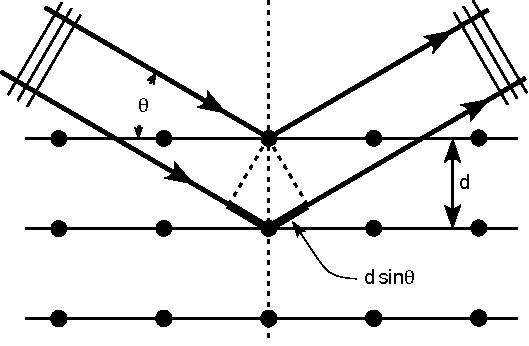
\includegraphics[width=0.30\textwidth]{difraction}
\label{fig:difraccion}
\end{figure}



\begin{equation}
\delta = \frac{2\pi d\sin{\theta}}{\lambda}
\label{equation:phase}
\end{equation}

Dado esto, si asumimos una onda sinusoidal normal, ambas ondas se anularán cuando su diferencia de fase sea $\delta = \pi$ y sea $\delta = 2\pi$. Claramente habrá interferencia constructiva y destructiva respectivamente para ángulos mayores si se agrega $2n\pi$ a cada desfase. Sin embargo, en este caso, para poder apreciar un buen patrón de difracción, consideramos que la longitud de onda de la onda incidente es del orden de magnitud de la distancia interplanar, por lo que se omitirán dichos casos. Además, si la onda se observa a una distancia $L$ del blanco en dirección perpendicular al plano del blanco, y a una distancia $R$ del blanco en dirección paralela a éste, asumiendo incidencia casi normal, es decir, $\theta \approx 0$, se tiene $\sin{\theta} \approx \frac{R}{L}$. Con todo esto, observaremos un patrón de interferencia constructiva que caracterizará el patrón de difracción cuando se cumpla la condición dada en la ecuación \ref{equation:mas}.\\

\begin{equation}
\frac{d\sin{\theta}}{\lambda} = \frac{dR}{L\lambda} = 1
\label{equation:mas}
\end{equation}

Ahora, sabiendo cuantificar la difracción para una onda normal, se puede caracterizar también la difracción de un haz de electrones. Para esto, solo es necesario tener en cuenta la relación de De Broglie para obtener la longitud de onda de un electrón libre con una energía $E$ determinada. La longitud de onda será entonces de la forma:\\

\begin{equation}
\lambda = \frac{p}{h} = \frac{\sqrt{2mE}}{h}
\label{equation:lambda}
\end{equation}

Donde claramente $h$ es la constante de Planck y $m$ es la masa del elctrón. Si asumimos además que cada electrón fue acelerado por un potencial eléctrico $V$, la ecuación \ref{equation:lambda} se reduce a:\\

\begin{equation}
\lambda = \frac{\sqrt{2meV}}{h}
\label{equation:lambda2}
\end{equation}

Ahora, la condición para el máximo en el patrón de difracción de electrones está dado por la unión de las ecuaciones \ref{equation:mas} y \ref{equation:lambda2}. En este caso, quedamos con la ecuación final para cuantificar la difracción de electrones: 

 \begin{equation}
\frac{dR}{L} = \frac{\sqrt{2meV}}{h}
\label{equation:lambda2}
\end{equation}

En este experimento tomaremos un blanco hecho de grafito el cual está compuesto de cristales pequeños irregularmente distribuidos. Estos cristales tienen celda unitaria hexagonal, por lo que habrán dos distancias interplanares importantes. Éstas distancias, la cuales tienen valores teóricos dados por la ecuación \ref{equation:carbono}, se pueden apreciar en la figura \ref{fig:carbono}.\\

\begin{equation}
d1 = 2.13 \textup{\AA} ; d2 = 1.23 \textup{\AA}
\label{equation:carbono}
\end{equation}

\begin{figure}[h]
\caption{Distancias interplanares en el grafito}
\centering
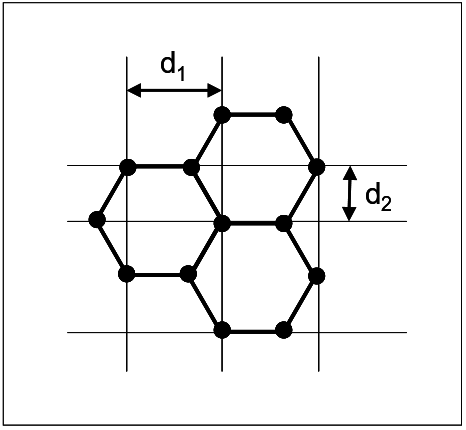
\includegraphics[width=0.30\textwidth]{carbono}
\label{fig:carbono}
\end{figure}

Dado que se hará incidir un haz de electrones de simetría axial contra el blanco de grafito, el patrón de difraccoión tendrá esta misma simetría proyectada sobre un plano perpendicular al eje determinado por el rayo. En este sentido, el patrón de difracción estará dado por círculos, por lo cual es mejor escribir la ecuación \ref{equation:lambda2} en términos del diámetro $D = 2R$ de dichos círculos:\\

 \begin{equation}
\frac{dD}{2L} = \frac{\sqrt{2meV}}{h}
\label{equation:final}
\end{equation} 


\section{\label{sec:level1}Montaje experimental}
Durante la presente práctica se utilizó un tubo de difracción de electrones que aceleraba electrones acelerados por un potencial y los hacía colisionar con un blanco de grafito. Dicho blanco sería también el motivo de estudio de este experimento pues se determinarían las distancias reticulares de la estructura hexagonal de este material. \\

El montaje se presenta en la figura a continuación. 
\begin{figure}
\centering
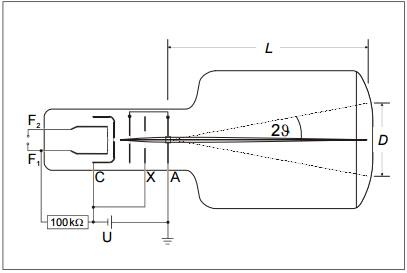
\includegraphics[width=0.7\linewidth]{montaje}
\caption[Vista esquemática del montaje experimental]{}
\label{fig:montaje}
\end{figure}

Como se expplicó en la introducción, el grafito tiene dos distancias interatómicas que son de interés medir, y por ello en la pantalla del detector se ven dos anillos de difracción, como se muestra en la figura de abajo.\\

\begin{figure}
\centering
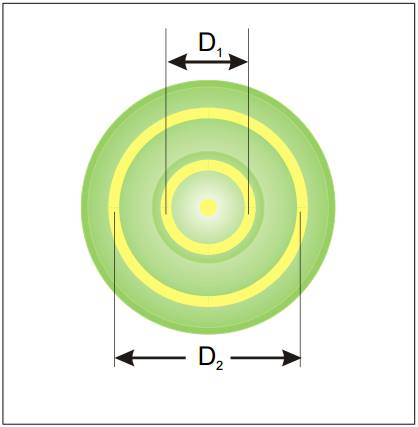
\includegraphics[width=0.7\linewidth]{Anillos}
\caption[Anillos de difracción en el detector.]{}
\label{fig:anillos}
\end{figure}


Para medir dichos anillos y su relación con el voltaje aplicado, se tomaron rangos desde 3.0 V hasta 5.0 V en aumentos de 0.5 V y se midieron los anillos respectivos. Sin embargo, los anillos tenían un ancho propio (0.2 cm) que puede ser generador de errores en la medición. Los anillos se midieron desde el centro del detector hasta el centro del anillo mismo con la mayor exactitud que pudo realizarse. \\


\section{\label{sec:level1}Resultados y An\'alisis}
En primer lugar se midieron los dos diámetros de los anillos y con base en ello se determinaron las demás variables. Los datos para los anillos se encuentran en la siguiente tabla. \\

\begin{table}[h!]
\begin{tabular}{|c|c|c|}
	\hline V (kV) & $ D_1 $ (cm) & $ D_2 $ (cm) \\ 
	\hline  3.0 &  2.96 &  5.14 \\ 
	\hline  3.5 &  2.85 &  4.78\\ 
	\hline  4.0 &  2.51 &  4.34\\ 
	\hline  4.5 &  2.40 &  4.12\\ 
	\hline  5.0 &  2.29 &  4.00\\ 
	\hline
\end{tabular} 
\caption{Mediciones de los anillos de difracción} 
\end{table}


Para cada valor de voltaje se puede encontrar el valor de la longitud de onda de los electrones correspondiente, usando la relación obtenida en el marco teórico: \[\lambda_n = \frac{d_n D_n}{2L} \] Con n=1,2 según sea la distancia interatómica que se quiera medir. Esto se puede ver en las siguientes dos tablas. Hay que anotar, como se mencionó anteriormente, que los anillos tenían un ancho considerable y al medir se pudieron cometer errores. \\

\begin{table}[h!]
\begin{tabular}{|c|c|c|c|}
	\hline V (KV) & $ D_1 $ (cm) & $ \lambda_1 $ (pm) & $ \lambda_{teo} $ (pm) \\ 
	\hline  3.00 &  2.96 &  23.23 &  22.39\\ 
	\hline  3.50 &  2.85 &  22.37 &  20.7\\ 
	\hline  4.00 &  2.51 &  19.7 &  19.39\\ 
	\hline  4.50 &  2.40 &  18.8 &  18.3\\ 
	\hline  5.00 &  2.29 &  17.97 &  17.34\\ 
	\hline
\end{tabular} 
\caption{Longitudes de onda para la primera distancia interatómica del grafito.} 
\end{table}

\begin{table}[h!]
\begin{tabular}{|c|c|c|c|}
	\hline  V (kV)& $ D_2 $ (cm) & $ \lambda_2 $ (pm) & $ \lambda_teo $ (pm)\\ 
	\hline  3.00 &  5.14 &  23.29 &  22.39 \\ 
	\hline  3.50 &  4.78 &  21.66 &  20.7 \\ 
	\hline  4.00 &  4.34 &  19.67 &  19.39 \\ 
	\hline  4.50 &  4.12 &  18.67 &  18.3 \\ 
	\hline  5.00 &  4.00 &  18.13 &  17.34 \\ 
	\hline
\end{tabular} 
\caption{Longitudes de onda para la segunda distancia interatómica} 
\end{table}

En cuanto a la determinación de las distancia interatómicas, se realizó una regresión lineal con los datos obtenidos para cada diámetro.\\

\begin{figure}[h!]
\centering
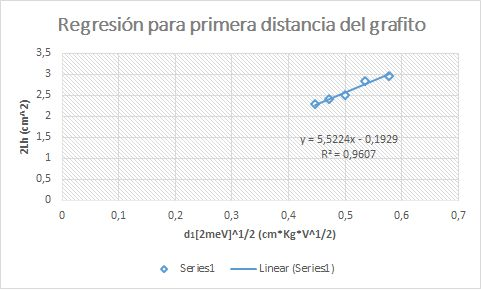
\includegraphics[width=0.7\linewidth]{regD1}
\caption[Regresión lineal para la primera distancia]{}
\label{fig:reg1}
\end{figure}

\begin{figure}[h!]
\centering
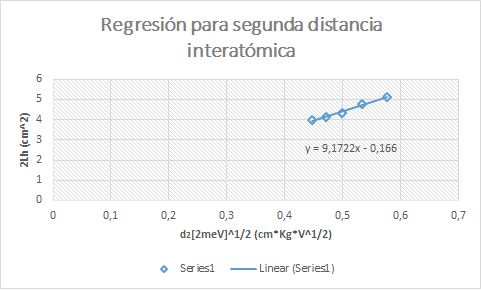
\includegraphics[width=0.7\linewidth]{RegD2}
\caption[Regresión lineal para la segunda distancia]{}
\label{fig:reg1}
\end{figure}


La primera pendiente, $ m_1 = 5.5224 $ da como resultado una distancia interatómica de $ d_1 = 2.015 \times 10^{-10} m $, las cuales están en unidades de $ \frac{m}{Kg*\sqrt{kV}} $ . Asimismo, la segunda pendiente $ m_2 = 9.1722 $ corresponde a $ d_2 = 1.148 \times 10^{-10} m $. Estos valores encajan correctamente con lo esperado según el marco teórico.\\

Ahora, para comprobar la constante de Planck, se usó la misma reggresión, pero en lugar de usar se despejó la constante y se reemplazaron las distancias por su valor teórico. Así pues, para el primer diámetro se encontró que $ h = 7.4 \times 10^{-34} Js$ y su valor correspondiente para el segundo diámetro medido fue de $ h=7.102 \times 10^{-34} Js $. \\

Estos valores encajan dentro del orden de magnitud, lo cual es bueno dado que se trata de una constante muy pequeña. Sin embargo, el valor teórico se encuentra razonablemente por debajo y se preferiría tener mejores valores dado el experimento. \\

\section{\label{sec:level1}Conclusiones}

Como se mencionó, el experimento podía dar paso a diferentes fuentes de error. Una fue el espesor propio de los anillos de difracción. Asimismo, cuando éstos iban a ser medidos, el uso del pie de rey resultaba poco preciso dado que la pantalla no era plana sino que tenía una curvatura. No obstante, las distancias interatómicas lograron ser medidas con considerable precisión.\\

El experimento muestra con claridad la dualidad onda-partícula del electrón. Dicho comportamiento se puede observar también en difracción de rayos X, y la misma medición se puede llevar a cabo, comprobando así el comportamiento. \\

Al hacer la regresión, la constante de Planck obtenida resultó estar dentro del orden de magnitud esperado, sin embargo se podría refinar mucho más el valro obtenido si se eliminaran los errores ya mencionados, que, si bien no presentaron mayor inconveniente para las primeras mediciones, al propagarlos seguramente afectaron la constatación de la constante. \\


\begin{thebibliography}{99} 
\bibitem{ondas} A.P. French,{\it vibraciones y ondas}{Editorial Reverté s.a.,1971}.\\ 
\bibitem{guia} Universidad de los Andes,{\it Guía: Difracción de electrones en red policristalina}{2015}.\\
\bibitem{} University of Saskatchewan,{\it X-RAY DIFFRACTION (DEBYE-SCHERRER METHOD)}{2004}
{De:http://physics.usask.ca/~bzulkosk/modphyslab/\\phys381manual/xray\_diffraction\_2004.pdf}\\
\end{thebibliography}


\end{document}
%
% ****** End of file apssamp.tex ******